\chapter{Manual del Usuario}
\label{anexo:manualUsuario}

\section{Verificaciones Iniciales}
\label{anexo:verificaciones}
Antes de poner en funcionamiento la planta verifique cada uno de los siguientes
items:

\tcbset{before app=\parfillskip 0pt}
\begin{tcolorbox}[title=Nivel de agua]
Si los tanques están vacíos, deben llenarse con agua hasta un 55\%
del total de su capacidad aproximadamente.

En el caso de contener agua, verifique que cada uno de los tanques no esté por
encima del 80\% ni por debajo del 20\%.
Puede transvasar el fluido de un tanque a otro utilizando el modo manual del
\gls{scada} o encendiendo manualmente las bombas.
\end {tcolorbox}
\begin{lattention}
En \textbf{modo automático}, si el nivel del tanque controlado desciende por
debajo del
20 \% o aumenta por encima del 80\% se detiene la planta automáticamente.

La planta no podrá volver a encenderse en modo automático hasta que se confirme
de parte del usuario que la planta no está en estado de emergencia (mediante el
\gls{scada} o poniendo a 1 la bandera \verb|MW1:X7|).
\end{lattention}

\begin{tcolorbox}[title=Válvulas manuales, breakable]
La planta cuenta con 6 válvulas manuales (ver \gls{pyid}).
Se describirá la posición de cada una
de ellas para un correcto funcionamiento de la planta.
 
 \begin{itemize}
  \item \textbf{Purgado de los tanques:} completamente cerradas.
  \item \textbf{Control de caudal del tanque de reserva \texttt{V1}:}
  la apertura de la válvula debe ser tal que el manómetro que está junto
  a la misma marque $0.5\,{Kg}/{cm^2}$. Esto nos asegura que el sistema está
  ecualizado.
  \item \textbf{Tiempo muerto \texttt{VDT}:} abierta, de tal manera que no
tenga efecto sobre la  planta la manguera del tiempo muerto.
  \item \textbf{Perturbación bomba llenado \texttt{VP1}:} totalmente cerrada,
para asegurar que el tanque controlado no se descargue más rápido de lo que se
llena.
  \item \textbf{Perturbación bomba vaciado \texttt{VP2}:} totalmente abierta.
  La bomba de vaciado debe perder rendimiento para poder ecualizar la planta
sin forzar una sobrepresión en la válvula \texttt{V1}.
 \end{itemize}
 \tcblower
 Estas válvulas están presentes para modificar el sistema y generar distintos
escenarios en la planta. Al modificar las características del sistema se deben
ajustar los valores del controlador.
\end {tcolorbox}

\begin{tcolorbox}[title=Presión de aire]
  Asegúrese que la presión de aire este regulada a $4\,bar$. Se debe controlar
  el correcto funcionamiento del filtro y regulador, realizando purgas en caso
de ser necesario.
 \tcblower
  Un filtro regulador, se utiliza de la siguiente manera:
 \begin{enumerate}
    \item Tener precaución de desconectar la manguera de aire a la válvula.
    \item Se conecta la línea de aire comprimido al regulador.
    \item Se visualiza el valor de presión en el manómetro
    \item Se desplaza hacia arriba la maneta de regulación y se gira hasta
      alcanzar el valor de presión deseado.
    \item Se vuelve a su posición original la maneta de regulación.
 \end{enumerate}
\end {tcolorbox}
%\todo{agregar filtro de aire}

\begin{lattention}
Nunca conectar la linea de aire comprimido de manera directa a la válvula,
sin el filtro regulador.
Puede dañar el electroposicionador de manera irreversible si la presión de aire
supera los $7\,bar$.
\end{lattention}

\begin{tcolorbox}[title=Motores]
Para poder encender los motores debemos asegurarnos que no están trabados.
Para verificarlo, se recomienda retirar la jaula que recubre los ventiladores
de los motores y hacer girarlos manualmente.
\end {tcolorbox}

\begin{lattention}
Luego de haber realizado todas las verificaciones debe enchufarse la planta a
la red eléctrica ($220\,V$, corriente alterna).
\end{lattention}

\section{Activación Manual de los Motores}
Se explican a continuación los pasos a seguir para activar, de modo manual, los
motores de la planta.
 \begin{lattention}
 La activación manual de los motores debe utilizarse exclusivamente en el caso
de que el sistema SCADA no responda.
Por favor, en caso de dudas consulte con el encargado del laboratorio.
\end{lattention}

%   \begin{enumerate}
%    \item Controlar que no estén trabados.
%    \item Energizar el sistema.
%    \item Conectar el aire, presión 4 bares.
%    \item Activar el relé manualmente que sea necesario.
%   \end{enumerate}

\begin{table}[H]
\centering
\renewcommand*{\arraystretch}{0.01}
\begin{tabular}{*{2}{m{0.45\textwidth}}}
\hline
% Fernando: Para mi es más importante esto que conectar la presión de aire.
% No podemos abrir la válvula así que no sirve de nada conectarla.
  Controlar que las bombas no estén bloqueadas.
  &\begin{center}
    \rule{0.4\textwidth}{0.3\textwidth}
    %\includegraphics[width=0.4\textwidth]
    %  {Cap5-SCADA/images/startUp.jpeg}
  \end{center}\\
% \hline
%     Conectar la planta a la linea de presión de aire. Presión 4 bares
%     &\begin{center}
%       \rule{0.4\textwidth}{0.3\textwidth}
%       %\includegraphics[width=0.4\textwidth]
% 	%{Cap5-SCADA/images/database.jpeg}
%     \end{center}\\
\hline
    Energizar el sistema. Activar el interruptor termomagnético ubicado dentro
    del tablero eléctrico.
    &\begin{center}
      \rule{0.4\textwidth}{0.3\textwidth}
      %\includegraphics[width=0.4\textwidth]
	%{Cap5-SCADA/images/database1.jpeg}
    \end{center}\\
\hline
    Activar manualmente el relé de la bomba correspondiente. En la imagen se
    puede apreciar la llave (color verde claro) que debe accionarse.
    &\begin{center}
      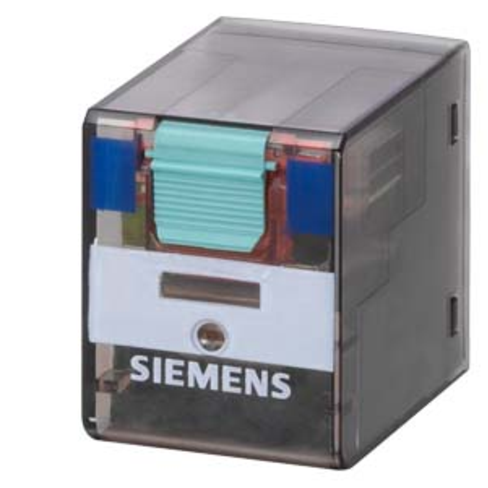
\includegraphics[width=0.3\textwidth]{Anexos/images/rele.pdf}
    \end{center}\\
\hline
\end{tabular}
\end{table}

Para mas información acerca del relé utilizado en esta planta, refiérase a la
hoja de datos del mismo.
Por favor, si tiene dudas acerca de como se acciona de manera manual, pida la
asistencia del encargado del laboratorio.
